\documentclass[a4paper,10.5pt]{article}
\usepackage{mathtools}
\usepackage{listings}
\usepackage{tikz-qtree}
\usepackage[utf8x]{inputenc}
\usepackage[font=small,format=plain,labelfont=bf,up,textfont=normal,up]{caption}
\usepackage[left=2.2cm,top=2cm,right=2.2cm,bottom=2cm,nohead,nofoot]{geometry}
\usepackage{wrapfig}
\usepackage{graphicx}
\usepackage{subcaption}
\setlength{\footskip}{25pt}
\usepackage{tikz}
\usepackage{amsmath,tikz}
\usetikzlibrary{shapes.geometric}
\usepackage{subcaption}
\usepackage{pgfplots}
\usepackage{filecontents}
\usepackage{algpseudocode}
\usepackage{algorithm}
\usepackage{subfig}
\usetikzlibrary{matrix}
\usetikzlibrary{shapes,arrows}
\renewcommand{\footnoterule}{%
  \kern -3pt
  \hrule width \textwidth height 0.5pt
  \kern 2pt
}
\tikzstyle{decision} = [diamond, draw, fill=white!20, 
    text width=6em, text badly centered, node distance=3cm, inner sep=1pt]
\tikzstyle{block} = [rectangle, draw, fill=white!20, 
    text width=5em, text centered, rounded corners, minimum height=3em]
\tikzstyle{line} = [draw, -latex']
\tikzset{
  treenode/.style = {align=center, inner sep=0pt, text centered,
    font=\sffamily},
 arn_n/.style = {treenode, circle, white,  font=\sffamily, draw=black,
    fill=black, text width=1.5em}
}
\usepackage{marginnote}
\usepackage{pgfgantt}
\usepackage{rotating}
\usepackage{pdflscape}
\usepackage{float}
\title{Random Number Generation using Genetic Programming\\ Design}
\author{Philip Leonard}
\date{}

\tikzset{
    maxfitnessorgen /.style={
        /pgfplots/execute at end plot visualization={\draw [current plot style, dashed] (@auxnode.center) -- ($(@auxnode.center)!10cm!(@auxnode.east)$);}
    },
    maxfitnessorgen nodestyle/.style={
        pos=1, inner sep=0pt, sloped, alias=@auxnode
    }
}

\begin{filecontents}{data.dat}
a,b,c,d,e,f,g,h
0,0,0,0, 0,27.99,51,0
1,0.7,1,0.8, 51,27.99,51,27.99
2, 1.3,2, 1.5
3, 2.9,3, 3.4
4, 3.2,4, 3.9
5, 3.3,5, 4.2
6, 3.4,6, 4.9
7,  3.7,7, 5.3
8, 3.9 ,8,5.6
9, 4.2 ,9, 5.7
10, 4.5,10, 6.2
11, 4.9, 11, 6.8
12, 5.3, 12, 6.9
13, 5.4,13, 7.1
14, 5.5,14, 7.3
15, 6.0,15, 7.6
16, 6.2,16, 8.9
17, 6.4,17, 9.2
18,  7.0 ,18, 10.1
19, 7.2,19, 10.8
20, 7.3,20, 11.8
21, 7.5,21, 12.9
22, 7.9,22, 13.8
23, 8.0,23, 14.7
24, 8.0,24, 15.3
25, 8.1,25, 16.9
26, 8.2,26, 17.2
27, 8.4,27, 18.3
28, 9.4,28, 18.9
29, 9.9,29, 20.9
30, 9.9,30,  22.4
31, 10.2,31, 23.9
32, 10.4, 32, 24.3
33, 10.7, 33, 25,9
34, 11.6, 34, 26.3
35, 11.7, 35, 27.4
36, 11.8, 36, 27.5
37, 12.7, 37, 27.6
38, 12.9, 38, 27.990
39, 13.2,
40, 13.9,
41, 13.9,
42, 14.5,
43, 14.8,
44, 15.2,
45, 16.9,
46, 17.4 ,
47, 18.2,
48, 18.9,
49, 19.3,
50, 20.5,
51, 21.2,

\end{filecontents}

\begin{document}
\maketitle
\begin{abstract}
This is the design document for the project; `Random Number Generation using Genetic Programming' by Philip Leonard, supervised by Dr David Jackson (primary supervisor) and Professor Paul Dunne (secondary supervisor). This document covers the summary of the project proposal, and primarily both the System and Evaluation Design. The last section covers the up to date plan for the project.\\\\
\textbf{Keywords:} Genetic Algorithm (GA), Genetic Programming/Program (GP), Pseudo Random Number Generator (PRNG), Random Number Generator (RNG), Entropy, Single Node Genetic Programming/Program (SNGP), Crossover, Mutation, Fitness proportionate reproduction (FPR).
\end{abstract}
\newpage
\tableofcontents
\section{Summary of Proposal}
The aim of this project is to Evolve a Random Number Generator using Genetic Programming, and Single Node Genetic Programming methodologies and to compare both approaches. Main objectives of the project are as follows;
\begin{description}
  \item[1)]
  \ \ \ Implement Koza's idea of Evolving a Random Number Generator using Genetic Programming from his paper \cite{kozarng} as a C program.
  \item[2)]
 \ \ \ Implement the same idea, but by using the Single Node Genetic Programming paradigm as described by Jackson in \cite{jacksonsngp2}, again as a C program.
  \item[3)]
  \ \  Finally compare both Genetic Programming methodologies, and then against common RNGs using evaluation methods designed in this document, in order to determine which approach to the problem is most effective. 
\end{description}
There are some changes to the initial specification regarding the proposed user manual for the software, and what the programs will output. Both GP and SNGP programs will produce files including; the prefix expression of the fittest individual in the population, the time it took to complete a run of the program, and both maximum and average entropies for each generation in that run. The user manual will then be more extensive than originally anticipated, as it will provide guidance on how this information should be used for practical and experimental use. The mechanics of the programs will also be discussed in detail in order to allow users to adapt the software.\\

As discussed in the specification document, research has been the dominating factor in preparing for this project. I began researching Genetic Algorithms \cite[p.1 - 24]{mitchell} and Genetic Programming \cite[p.1 - 35]{introgp} \cite[p.73 - 191]{kozagpbook} topics. Since then I have researched more specifically into Genetic Programming, including a C implementations of Multiplexer Problem described in \cite{kozamux}. So far the focal point of my research has been around the paper by Koza \cite{kozarng}, which is the inspiration for the implementation of this project using GP. Since creating the Specification document, the next key bit of research has been into SNGP, using \cite{jacksonsngp2} to formulate the design for the second objective. 

\section{Design}
\subsection{System Design}

%- Discuss how not using OO approach. How for GP and SNGP will each only require a single C program file.\\

Both GP and SNGP approaches will be implemented in the C programming language. C will provide computational leverage over other programming languages whilst also providing effective ways of dealing with program structures and manipulating memory, making it a highly suitable candidate for the job. Both implementations will each require a single C program file, and will require no parallelism/threading because of GP and SNGPs sequential problem solving style. As a result of these characteristics, the best approach to the design of the project is to use a traditional methodology, describing it at a functional level. This includes a written design of the components, flow charts and the respective pseudocode of the key methods for both GP and SNGP solutions. Finally the evaluation design will encompass the test methods, conditions and comparison techniques used in order to evaluate and compare both approaches, and to pit them against other widely used RNGs.

%- Discuss the anticipated components of the software\\
\subsubsection{GP Approach}
This section covers the design for the GP approach of evolving a RNG. 

The goal is to genetically breed a RNG to randomise a sequence of binary digits. The input to the RNG will be the sequence $J$, which will run from $i = 1$ to $2^{14}$. The output will be a sequence of random binary digits of size $J$. The binary digit at location $i$ will be determined by the value of the LSB\footnote{Least Significant Bit. The lowest (furthest right) bit in a binary sequence determining whether the number is odd or even.} from the output of the RNG on the $i^{th}$ input. For example, given a RNG which outputs $12$ on the $5^{th}$ iteration (input $i = 5$), the value of the $5^{th}$ digit in the binary sequence will be $0$, as the LSB of 1100 ($12_{10} = 1100_2$) is 0. 

\begin{wrapfigure}{r}{.4\textwidth}
\caption{RNG binary tree}
\label{fig:simplebintree}
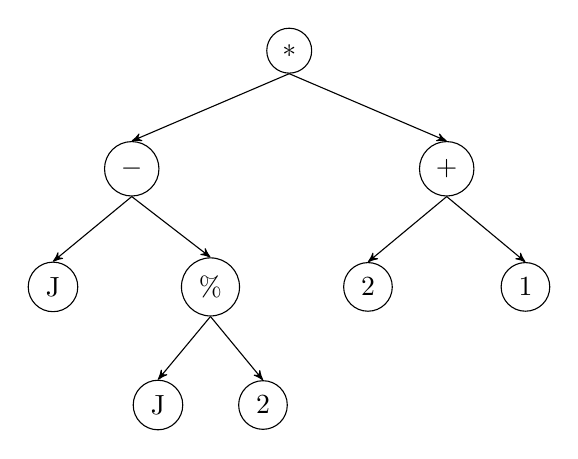
\begin{tikzpicture}[->,>=stealth',level/.style={sibling distance = 4cm/#1,
  level distance = 1.5cm}] 
\node[circle,draw](z){$*$}
 child{
    node[circle,draw]{$-$} child{node[circle,draw] {J}} child{node[circle,draw] {$\%$} child{node[circle,draw] {J}}  child{node[circle,draw] {2}}} }
  child{
    node[circle,draw]{$+$} child{node[circle,draw] {2}} child{node[circle,draw] {1}} };
\end{tikzpicture}
\end{wrapfigure}

As explained in \cite[p.19-27]{introgp} to begin designing a GP, the first step is to define the set of terminals and the set of functions, of which the program trees will be comprised of. The terminal set will be; \begin{center}$T = \{J,\ \Re\}$\end{center} $J$ as already discussed will be the value in the sequence 1 to $2^{14}$, and $\Re$ will represent a small random integer constant from the set $\{0, 1, 2, 3\}$. The set $F$ is our function or operator set; \begin{center}$F = \{+, -, *, /, \%\}$\end{center}In this set, $/$ is the protected integer quotient function and $\%$ is the protected modulus function, where both use the protected division function that returns 1 when attempting to divide by zero, and otherwise returns the normal quotient. All the terminals have an arity of 0, and all the functions have an arity of 2.

\begin{text}The next step is to define the structure of the programs. Members of the population will be represented as binary trees, in the form of prefix expressions. Take for example the expression; \end{text}
\begin{equation*}*\ -\ J\ \%\ J\ 2\ +\ 2\ 1 \end{equation*} 
This prefix expression can be represented as the binary tree in figure \ref{fig:simplebintree}. And vice versa, the prefix expression above can be generated from a pre-order traversal of the binary tree in figure \ref{fig:simplebintree}. For experimentation, the user will initially define the major parameters of the GP run. These parameters are defined in figure \ref{inputparam} below;

\begin{figure}[H]
\centering
\caption{Input parameters}
\label{inputparam}
\begin{tabular}{l*{6}{l}r}
Data Type             & Input description\\
\hline
Integer & Population size\\
Integer & Maximum number of generations\\
Integer & Maximum initial program depth and maximum crossover program depth\\
Double & Fitness proportionate reproduction to crossover operation balance\\
Double & Internal to external node crossover probabilities\\
Double & Target fitness value\\
\end{tabular}
\end{figure}

Now we have defined the parameters, the terminals $T$, the functions $F$, and the structural representation of the programs, the next step for the GP is to use these definitions to enumerate an initial random population of programs.

Defined by the user, the GP will generate a population of the given size, where each program in the population has a maximum initial tree depth of the given size. In order to generate a wide and genetically diverse initial population, in \cite[p.11-14]{introgp} Koza suggests the even combination of both ``grow" and ``full" methods to generate program trees known as the ``ramped half and half method". In the full method, trees are filled on all branches right up to the maximum initial depth. This is done by recursively choosing nodes from $F$ to populate the tree until the depth is one less than the maximum. The remaining nodes are filled as randomly selected elements of $T$. The grow function on the other hand randomly selects an element from the set $F \cup T$ until all branches are terminated with an element of $T$ (still limited by the maximum depth). If the selected element is a function then it has an arity of 2, so two more branches are recursively generated. Otherwise the selected element is a terminal which has an arity of 0, and therefore no further leaf nodes are generated. This allows for a range of tree shapes and sizes all the way from a single terminal node program such as $J$, all the way up to a program which would be produced by the full function. Using this ramped half and half method, we can obtain half a population of large programs, and another half of programs with varying shapes and sizes.

Now that the GP has obtained an initial random population, it will evaluate each program and calculate it's corresponding fitness. A discussed above, the output of the RNG is a sequence of random binary digits of length $J$. To calculate the output, we must run through the sequence $J$ from $I = 1$ to $2^{14}$ substituting the occurrences of $J$ in the program with $i$. The LSB of the output given $J = i$ corresponds to the value in the binary sequence at position $i$. The GP will then calculate the binary output sequence for each RNG in the population. 

Now that the GP has evaluated every RNG, it must use a fitness function to calculate the fitness for each RNG given its respective output. In order to measure how ``random" the output is from a RNG, their are a variety of techniques at our disposal. In this GP, we shall use the entropy of a given output to correspond to the fitness of that RNG. The entopy of a sequence of binary digits, is the equality in the occurrence of a set of binary subsequences of length $h$ in that sequence. The entropy calculation for all possible $2^h$ binary subsequences of length $h$ is;
\begin{equation*}
E_{h} = - \sum_{j} P_{(hj)}\ \log_2\ P_{(hj)}
\end{equation*}
Here $j$ ranges over all possible subsequences of length $h$ in the binary sequence (the RNG output in this case). For example take the binary sequence $1111$, and take $h = 2$. Here $E_2 = 0$ as there are 4 possible binary subsequences of length $2$; $\{00, 01, 10, 11\}$, and only $11$ occurs in the sequence $1111$. Therefore $1 \log_2 1 = 0$, and for the 0 probabilities of the other sub strings; $0 \log_2 0 = 0$. The negated sum of these values is 0, and therefore the sequence $1111$ achieves the minimal entropy for sub sequences of length $2$. Take another binary sequence $10011$, for $h = 2$. This sequence obtains the maximum entropy for $E_2$, as the binary sub sequences of length $2$; $\{00, 01, 10, 11\}$ occur with equal probabilities; $\{0.25, 0.25, 0.25, 0.25\}$ so the calculation of the entropy would be; 
\begin{eqnarray*}
E_{2} &=& -(0.25 \log_2 0.25 + 0.25 \log_2 0.25 + 0.25 \log_2 0.25 + 0.25 \log_2 0.25)
\\ &=& -(-0.5 + -0.5 + -0.5 + -0.5)
\\ &=& 2
\end{eqnarray*}
Therefore in order to achieve maximum entropy for $E_h$, all probabilities for all $2^h$ binary sub sequences of length $h$ must be equal to $\frac{1}{2^h}$.

To calculate the entropy for the output of every RNG, I want to evaluate it for more than one binary sub sequence length. This is achieved by calculating the summation of the formula above for $E_h$ but over a range of lengths of $h$ from 1 to $N_{max}$; 

\begin{equation*}
E_{total} = \sum_{h = 1}^{N_{max}} \left[ - \sum_{j} P_{(hj)}\ \log_2\ P_{(hj)} \right]
\end{equation*}
The maximum possible entropy value for sub sequences from 1 to $N_{max}$ can be calculated using the following sum;
\begin{eqnarray*}
E_{max} &=& \sum_{i = 1}^{N_{max}} i
\\ &=& \frac{N_{max}(N_{max} + 1)}{2}
\end{eqnarray*}
In my GP, I shall be using sub sequences of lengths 1 to 7, so $N_{max} = 7$. This will give me the maximum entropy and therefore the maximum fitness of 28;
\begin{eqnarray*}
E_{max} &=& \sum_{i = 1}^{7} i
\\ &=& \frac{7 \cdot (7 + 1)}{2}
\\ &=& 28
\end{eqnarray*}

\newpage
\begin{wrapfigure}{r}{.3\textwidth}
\caption{GP flowchart}
\label{simpleflow}
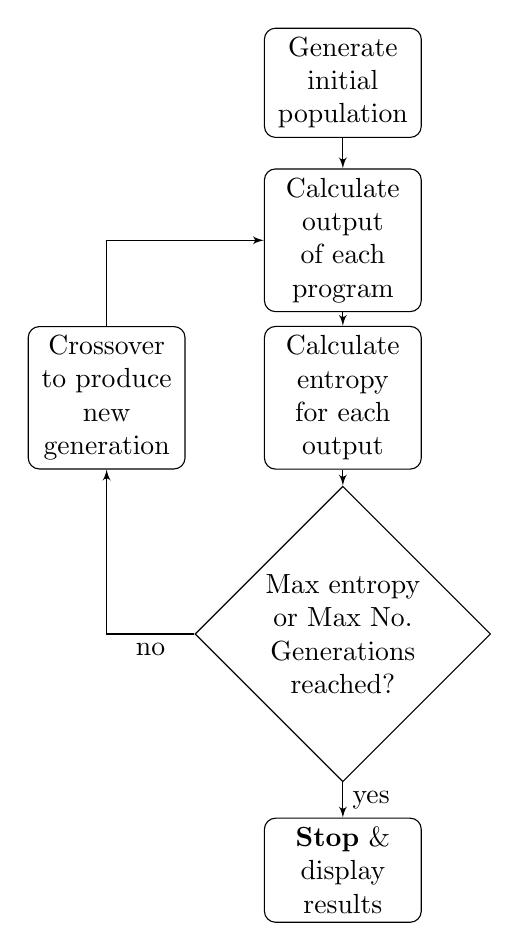
\begin{tikzpicture}[node distance = 2cm, auto]
    % Place nodes
    \node [block] (init) {Generate initial population};
    \node [block, below of=init] (identify) {Calculate output of each program};
    \node [block, below of=identify] (evaluate) {Calculate entropy for each output};
    \node [block, left of=evaluate, node distance=3cm] (update) {Crossover to produce new generation};
    \node [decision, below of=evaluate] (decide) {Max entropy or Max No. Generations reached?};
    \node [block, below of=decide, node distance=3cm] (stop) {\textbf{Stop} \& display results};
    % Draw edges
    \path [line] (init) -- (identify);
    \path [line] (identify) -- (evaluate);
    \path [line] (evaluate) -- (decide);
    \path [line] (decide) -| node [near start] {no} (update);
    \path [line] (update) |- (identify);
    \path [line] (decide) -- node {yes}(stop);
\end{tikzpicture}
\end{wrapfigure}
Now that the fitness function has been defined. The entropy for every RNG's output is calculated, for sub sequences of lengths 1 to 7.
In the C implementation, each program (RNG) will be stored in an individual struct. Each struct will contain; the RNG code/prefix expression, the program length, the output binary sequence, the scalar entropy break down for each of the sub sequence lengths of $h$ from 1 to $N_{max} = 7$ and the total fitness (the sum of these scalar entropies). So far in the design, all of these pieces of information have been defined. The population of all these structs are contained in another ``population struct" of the size defined by the user. Representing the programs and the population like this allows for easy manipulation and portability between methods in the GP.


Figure \ref{simpleflow} is a simple flow chart representation for the GP. At this point we have defined the first 3 operations. The 4th step is a Boolean decision which determines the continuation or termination of the GP, based on one or both of the two following termination criteria being satisfied;
\begin{description}
  \item[1)]
  \ \ \ The program in the population with the maximum fitness/entropy is greater than or equal to the user defined target fitness value, or
  \item[2)]
 \ \ \ The current generation number is equal to the user defined maximum number of generations.
\end{description}

If neither of these criteria are met, then the next stage is to prepare a modified population for the next generation. If one or both of these criteria are met, the GP will terminate. Regardless of which outcome happens, data is gathered for that particular run and is saved to a text file in the format of a CSV\footnote{Where values are delimited using commas i.e. $w,\ x,\ y,\ z, ...$}(Comma Separated Values) file. Each output and it's type are defined in figure \ref{outputparam} below;

\begin{figure}[H]
\centering
\caption{Output data}
\label{outputparam}
\begin{tabular}{l*{6}{l}r}
Data Type             & Output description\\
\hline
Integer & Generation number\\
Double & Generation run time in seconds \& hundredths of a second \\
Double & Total entropy/fitness of fittest candidate\\
Double & Entropy for subsequence size 1 of fittest candidate\\
\ \ \ \ $\vdots$ & \ \ \ \ \ \ \ \ \ \ \ \ \ \ \ \ \ \ \ \ \ \ \ \ $\vdots$\\
Double & Entropy for subsequence size 7 of fittest candidate\\
Boolean & Entropy of fittest candidate is $\geq$ target fitness?\\
String & Prefix expression for fittest candidate\\
\end{tabular}
\end{figure}

\begin{text}
This comma separated data will be appended to the text file for each generation of the GP (each preceded with a return line character). For example, after 3 generations the file could look like the following\footnote{The purpose of the example data here is to display its format, and the entropy values are not correct for the corresponding prefix expressions};
\end{text}

\begin{lstlisting}
1, 12.51, 1.0, 1.9, 0.8, 0.0, 0.0, 0.0, 0.0, 3.7, FALSE, +J2
2, 15.23, 1.0, 2.0, 2.8, 2.1, 0.2, 0.0, 0.0, 8.3, FALSE *%J2-J1
3, 24.32, 1.0, 2.0, 3.0, 4.0, 2.9, 1.2, 0.0, 14.1, FALSE *-J%J2+21
\end{lstlisting}

\begin{text}
Gathering and storing data in this way will aid in the evaluation of the GP against SNGP (where data will be gathered in a similar manner). Storing it in the CSV format will allow me to easily import the data into Microsoft Excel, MATLAB and \LaTeX \ in order to conduct statistical analysis and construct graphical representations. Including this as a component of the software will also allow future users to conduct their own evaluation and analysis. The user manual will also contain information and instructions on how to manipulate this data in the software mentioned above. The files created will contain a time stamp in their name so that a user can conduct multiple runs without having to worry about the data from the last run being overwritten. This will aid evaluation later on.
\end{text}

The final process in the GP to define is the genetic operation which shall be used. Two main genetic operations used in GP are mutation and crossover \cite[p.15-17]{introgp}. Both operate by altering program trees in different ways in order to create offspring programs. In this GP, I will be using the subtree crossover operation alone, and I will not be implementing subtree mutation in order to conserve computing time\footnote{Subtree mutation requires the generation of new subtrees which can prove to be computationally intensive, especially when mutation probability is high}.  

Subtree crossover works by taking two parent program trees and joining them to create two offspring programs. This is done by selecting a crossover point (node) in each parent tree. Both of the subtrees at the root of the crossover point are then swapped to generate the two new offspring. Crossover point selection can be at any node in the tree including leaf (in this case terminal) nodes. For this GP, one of the user inputs to the program in figure \ref{inputparam} on page \pageref{inputparam} is the probability divide of selection of internal to external nodes. In \cite[p.114]{kozagpbook}, Koza describes the benefits of using a 90\% internal (function) and 10\% external (terminal) split, saying that it ``promotes the recombining of larger structures" so that simple swapping of terminals like that of point mutation is less probable.

Figure \ref{fig:crossover} shows an example of subtree crossover for the two parent trees;
\begin{equation*}\{* \ \underbrace{-}_{\mathclap{\text{crossover point}}} J \ \% \ J \ 2 \ + \ 2 \ 1 \}\text{ \textbf{and} } \{\% \ * \ 2 \ 2 \ / \ J \ \underbrace{*}_{\mathclap{\text{crossover point}}} \ 3 \ J \}
\end{equation*}
which produce the offspring; 
\begin{equation*}\{* \ * \ 3 \ J \ + \ 2 \ 1\} \text{ \textbf{and} } \{* \ * \ 2 \ 2 \ / \ J \ - \ J \ \% \ J \ 2 \}
\end{equation*}

\begin{figure}[H]
\caption{Example of subtree crossover}
\label{fig:crossover}

\begin{subfigure}[h!]{1\textwidth}
\caption{\textbf{Parents}}
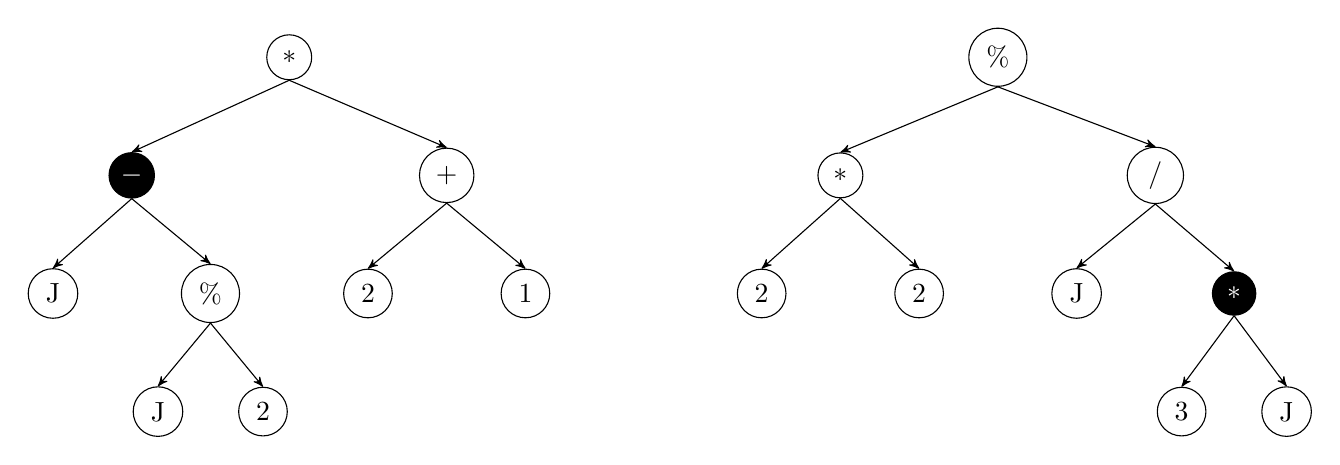
\begin{tikzpicture}[->,>=stealth',level/.style={sibling distance = 4cm/#1,
  level distance = 1.5cm}] 

\node[circle,draw](z){$*$}
 child{
    node[circle, draw, arn_n]{$-$} child{node[circle,draw] {J}} child{node[circle,draw] {$\%$} child{node[circle,draw] {J}}  child{node[circle,draw] {2}}} }
  child{
    node[circle,draw]{$+$} child{node[circle,draw] {2}} child{node[circle,draw] {1}} };
\begin{scope}[xshift=9cm]
\node[circle,draw](z){$\%$}
 child{
	node[circle,draw]{$*$} child{node[circle,draw] {2}} child{node[circle,draw] {2}} }   
  child{
     node[circle,draw]{$/$} child{node[circle,draw] {J}} child{node[circle,draw, arn_n] {$*$} child{node[circle,draw] {3}}  child{node[circle,draw] {J}}} };

\end{scope}
\end{tikzpicture}
\end{subfigure}

\begin{subfigure}[h!]{1\textwidth}
\centering
\caption{\textbf{Offspring}}
\begin{tikzpicture}[->,>=stealth',level/.style={sibling distance = 4cm/#1,
  level distance = 1.5cm}] 
\node[circle,draw](z){$*$}
 child{
    node[circle, draw]{$*$} child{node[circle,draw] {3}}  child{node[circle,draw] {J}} }
  child{
    node[circle,draw]{$+$} child{node[circle,draw] {2}} child{node[circle,draw] {1}} };

\begin{scope}[xshift=9cm]
\node[circle,draw](z){$*$}
 child{
	node[circle,draw]{$*$} child{node[circle,draw] {2}} child{node[circle,draw] {2}} }   
  child{
     node[circle,draw]{$/$} child{node[circle,draw] {J}}  child{
    node[circle, draw]{$-$} child{node[circle,draw] {J}} child{node[circle,draw] {$\%$} child{node[circle,draw] {J}}  child{node[circle,draw] {2}}} } };
\end{scope}
\end{tikzpicture}
\end{subfigure}
\end{figure}

In figure \ref{inputparam} on page \pageref{inputparam}, there is a parameter ``Fitness proportionate reproduction to crossover operation balance". This input determines the split between Fitness proportionate reproduction (FPR) and crossover.  FPR is where both parents are selected for crossover relative to their fitness. In the regular crossover selection, one of the parents is selected relative to their fitness and the other is selected with an equal probability amongst the rest of the population. The following equation calculates the selection probability for the $i^{\text{th}}$ individual in the population (used for selecting both parents in FPR and one in crossover);\\
\begin{center}
\noindent\begin{minipage}{.3\linewidth}
\begin{equation*}
p_i = \Bigg( \frac{f_i}{\sum_{x=1}^{|P|} f_x} \Bigg)
\end{equation*}
\end{minipage}%
\begin{minipage}{.2\linewidth}
where;
\end{minipage}
\begin{minipage}{.3\linewidth}
$p_i$ - selection probability of $i$\\
$f_i$ - fitness value of $i$\\
$f_x$ - fitness value of $x$\\
$|P|$  - population size
\end{minipage}
\end{center}

As Lapante explains in \cite[p.63]{lapantebio}, we can imagine a roulette wheel where members of the population with higher fitnesses (i.e. probabilities) are given greater chunks. For FPR, both parents are selected at random relative to their probabilities (size of chunk on the roulette wheel). For crossover (in this case as described by Koza in \cite[p.41]{kozarng}), one of the parents is selected in this manner and the other is selected where the probabilities of every member in the population is equal. A typical balance between the two methods is 90\% crossover and 10\% FPR. In this case, given a population of size 500, our new population is generated by conducting $500/2 * 0.9 = 225$ crossover operations and $500/2 * 0.1 = 25$ FPR operations. 

If the proportion of FPR is too high, we are at risk of reducing genetic diversity, and creating two segregated sub populations similar to the biological effects of Allopatric or Peripatric Speciation.
If this occurred in the GP, one population could be full of the fittest candidates, and the other contains the least fittest, and interbreeding could occur only rarely across the two populations.

Now that the GP has generated a new \emph{evolved} population, it returns back to step 2 in figure \ref{simpleflow} on page \pageref{simpleflow}. This process continues until one or both of the termination criteria are met as discussed above.\\

Above is a literal design of the GP, covering all the major aspects of the operations in detail. Using the definitions above, a pseudocode can be created for the key methods in figure \ref{simpleflow} on page \pageref{simpleflow} which bears a closer functional resemblance to the actual C implementation of the GP. I will use this pseudocode in Algorithms 1 to 6 in order to aid me in the implementation stage.

\begin{algorithm}[H]
  \caption{Generate-Initial-Population($P_{s}$, $M_{id}$)}
  \textbf{Input:} Population size $P_{s}$ and Maximum initial depth $M_{id}$\\
  \textbf{Output:} Population $P$ of randomly generated programs of size $P_s$\\
  \begin{algorithmic}[1]
    \State $i \gets 1$
    \For {$i$ to $P_{s}$} 
	\If {$i \mod 2 == 0$}
		\State $grow \gets true$
	\Else
		\State $grow \gets false$
	\EndIf
	\State $partialTree \gets \varepsilon$
	\State $T \gets$ Create-Tree($partialTree$, $grow$, $M_{id}$)
	\State add $T$ to population $P$
    \EndFor	
\State \textbf{return} $P$
  \end{algorithmic}
\end{algorithm}

\begin{algorithm}[H]
  \caption{Create-Tree($partialTree_i$, $grow$, $d$)}
  \textbf{Input:} Boolean value $grow$ to select grow or full function and Integer current depth $d$, and the tree with so far $partialTree_i$ with pointer $i$\\
  \textbf{Output:} Recursively selects functions or terminals to produce a prefix expression\\
  \begin{algorithmic}[1]  
  \If {$depth == 1$}
	\State $node \gets $ random terminal
  \Else
	\If {$grow == true$}
		\State $node \gets $ random function or terminal
		\State add node to $partialTree_{i+1}$
	\Else
		\State $node  \gets $ random function or terminal
		\State $partialTree_{i+1} \gets node$
		\If {$node$ is a function}
			\For {$i \gets 1$ to arity of function}
				\State $partialTree \gets $ Create-Tree($partialTree$,  $grow$, $depth-1$)
			\EndFor
		\EndIf
     	\EndIf
  \EndIf  
\State \textbf{return} $partialTree$
  \end{algorithmic}
\end{algorithm}

\begin{algorithm}[H]
  \caption{Calculate-Output($T$, $J$)}
  \textbf{Input:} Tree prefix code $T$, Integer $J$\\ 
  \textbf{Output:} Binary sequence $O$ of size $J$\\

  \begin{algorithmic}[1]
  \For {$i \gets 0$ to $J$}
	\State $output \gets$ Evaluate-Tree($T_0$, $i$)
	\State $O[i] \gets output\mod 2$
 \EndFor
\State \textbf{return} $O$
  \end{algorithmic}
\end{algorithm}

\begin{algorithm}[H]
  \caption{Evaluate-Tree($T_{x}$, $currentJ$)}
  \textbf{Input:} Tree prefix code $T_{x}$ with a pointer to the node $x$, Integer $currentJ$ which is the value of $J$ in this instance\\ 
  \textbf{Output:} Integer output of the subtree\\ 
	
  \begin{algorithmic}[1]
  \State $node \gets T_{x+1}$
  \If {$node$ is $+$}
	\State \textbf{return} Evaluate-Tree($T_{x}$, $currentJ$) $+$ Evaluate-Tree($T_{x}$, $currentJ$)
  \ElsIf {$node$ is $-$}
	\State \textbf{return} Evaluate-Tree($T_{x}$, $currentJ$) $-$ Evaluate-Tree($T_{x}$, $currentJ$)
  \ElsIf {$node$ is $*$}
	\State \textbf{return} Evaluate-Tree($T_{x}$, $currentJ$) $*$ Evaluate-Tree($T_{x}$, $currentJ$)
  \ElsIf {$node$ is $\%$}
	\State \textbf{return} Evaluate-Tree($T_{x}$, $currentJ$) $\%$ Evaluate-Tree($T_{x}$, $currentJ$)
  \ElsIf {$node$ is $/$}
	\State \textbf{return} Evaluate-Tree($T_{x}$, $currentJ$) $/$ Evaluate-Tree($T_{x}$, $currentJ$)
  \ElsIf {$node$ is $J$}
	\State \textbf{return} $currentJ$
  \Else
	\State \textbf{return} $node$ \Comment{we know $node$ must be $\Re$, so return it's value}
  \EndIf
  \end{algorithmic}
\end{algorithm}

\begin{algorithm}[H]
  \caption{Fitness-Function($O$)}
  \textbf{Input:} Tree binary sequence output $O$\\
  \textbf{Output:} Fitness value $E_{total}$, and scalar entropies $E_1, E_2, ..., E_7$ corresponding to the output $O$ (which in turn corresponds to a tree/RNG)\\ 
  \begin{algorithmic}[1]
   
   \State $E_{total} \gets 0$
   \For {$h \gets 1$ to 7} \Comment{this algorithm represents $E_{total} = \sum_{h = 1}^{7} \left[ - \sum_{j} P_{(hj)}\ \log_2\ P_{(hj)} \right]$}
	\State $F \gets \emptyset$
	\State $totalOcc \gets 0$\\
	\State $j \gets 2^{h-1}$ 
	\If {$h == 1$} \Comment{we want to include 0 as a binary sequence of length 1}
		\State $j \gets 0$
	\EndIf\\
	\For {$j$ to $2^h - 1$} \Comment{this is for all numbers of binary sequence length $h$}
		\State $occurrence \gets 0$\\
		\For {$i \gets 0$ to $|O|$} 
			\If {$j_2$ occurs at shift $i$ in $O$} \Comment{$j_2$ is $j$ in base 2}
				\State $occurrence \gets occurrence + 1$
			\EndIf
		\EndFor
		\State $F \cup \{(j_2, occurrence)\}$ 
		\State $totalOcc \gets totalOcc + occurrence$
	\EndFor
	\State $E_h \gets 0$ \Comment{calculating entropy value for subsequence size $h$}
	\For {$\forall x \in F$} 
		\State $E_h \gets E_h + \left(-1 * \left( \frac{x.occurrence}{totalOcc} \log_2 \frac{x.occurrence}{totalOcc}\right)\right) $	
	\EndFor

	\State $E_{total} \gets E_{total} + E_h$
    \EndFor
    \State \textbf{return} $E_{total}, E_1, E_2, ..., E_7$
  \end{algorithmic}
\end{algorithm}

\begin{algorithm}[H]
  \caption{Crossover-Operation($T^1$, $T^2$, $i_1$, $j_1$ $i_2$, $j_2$)}
  \textbf{Input:} Two parent trees $T^1$ and $T^2$ with their respective crossover subtrees from $i_1$ to $j_1$ and from $i_2$ to $j_2$\\
  \textbf{Output:} Two children trees $T^1_{new}$ and $T^2_{new}$.\\
  \begin{algorithmic}[1]
  \State $T^1_{new} \gets \emptyset$
  \State $T^2_{new} \gets \emptyset$\\
  \For {$x \gets 0$ to $i_1$}\Comment{copying up to crossover point in $T^1$}
    \State $T^1_{new} \gets T^1_{new} + T^1_{x}$ \Comment{$ T^1_{x}$ denotes the character/node at position $x$ in $T^1$}
  \EndFor
    \For {$y \gets i_2$ to $j_2$}\Comment{copying crossover subtree in $T^2$ into $T^1_{new}$}
    \State $T^1_{new} \gets T^1_{new} + T^2_{y}$ \Comment{$ T^2_{y}$ denotes the character/node at position $y$ in $T^2$}
  \EndFor
  \For {$z \gets j_1+1$ to $|T^1|$} \Comment{copying the rest of $T^1$ after the subtree into $T^1_{new}$}
    \State $T^1_{new} \gets T^1_{new} + T^1_{z}$ \Comment{$ T^1_{z}$ denotes the character/node at position $z$ in $T^1$}
  \EndFor\\
  
  \For {$x \gets 0$ to $i_2$}\Comment{copying up to crossover point in $T^2$}
    \State $T^2_{new} \gets T^2_{new} + T^2_{x}$ \Comment{$ T^2_{x}$ denotes the character/node at position $x$ in $T^2$}
  \EndFor
    \For {$y \gets i_1$ to $j_1$}\Comment{copying crossover subtree in $T^1$ into $T^2_{new}$}
    \State $T^2_{new} \gets T^2_{new} + T^1_{y}$ \Comment{$ T^1_{y}$ denotes the character/node at position $y$ in $T^1$}
  \EndFor
  \For {$z \gets j_2 + 1$ to $|T^2|$}\Comment{copying the rest of $T^2$ after the subtree into $T^2_{new}$}
    \State $T^2_{new} \gets T^2_{new} + T^2_{z}$ \Comment{$ T^2_{z}$ denotes the character/node at position $z$ in $T^2$}
  \EndFor\\
\State \textbf{return} $T^1_{new}$, $T^2_{new}$ 

  \end{algorithmic}
\end{algorithm}

\begin{algorithm}[H]
  \caption{Output-Data($g_n$, $f_{max}$, $E_{av}$, $E_1$, $E_2$, $E_3$, $E_4$, $E_5$, $E_6$, $E_7$, $T$, $F$, $found$)}
  \textbf{Input:} $g_n$ generation number, $E_{total}$, $E_1$, ..., $E_7$  total and scalar entropies of fittest candidate, $E_{av}$ average entropy across all candidates,  $T$ prefix expression of fittest candidate, the file $F$ and a boolean value $found$ whether the solution has been found in that run\\
  \textbf{Output:} Write data to file, if successful then return 1, if not then return -1\\
  \begin{algorithmic}[1]
   	\State $line \gets g_n$, $E_{total}$, $E_{av}$, $E_1$, $E_2$, $E_3$, $E_4$, $E_5$, $E_6$, $E_7$, $T$, $found$ \textbackslash n
   	\State open($F$)
	\If {write($line$, $F$) == true}
		\State close($F$)
		\State \textbf{return} 1
	\Else
		\State close($F$)
		\State \textbf{return} -1
	\EndIf
	
  \end{algorithmic}
\end{algorithm}

\newpage

\subsubsection{SNGP Approach}

The following section of this document is concerned about the design of the SNGP implementation of evolving a RNG by means of Genetic Programming. To do this, I shall be using both \cite{kozarng} by Koza and \cite{jacksonsngp2} by Jackson.

Single Node Genetic Programming is similar to regular Genetic Programming in many ways, but differs in a few crucial aspects, giving rise to considerable efficiency and solution rate boosts over GP. For this reason, the design of the SNGP methodology need not be as extensive as that in section 2.1.1, but rather more to the point in terms of defining the approaches differences in comparison to GP. In \cite[p.50-51]{jacksonsngp2} Jackson describes the SNGP model in the following way;

\begin{wrapfigure}[39]{h}{.4\textwidth}
\label{simpleflowsngp1}
\caption{SNGP flowchart}
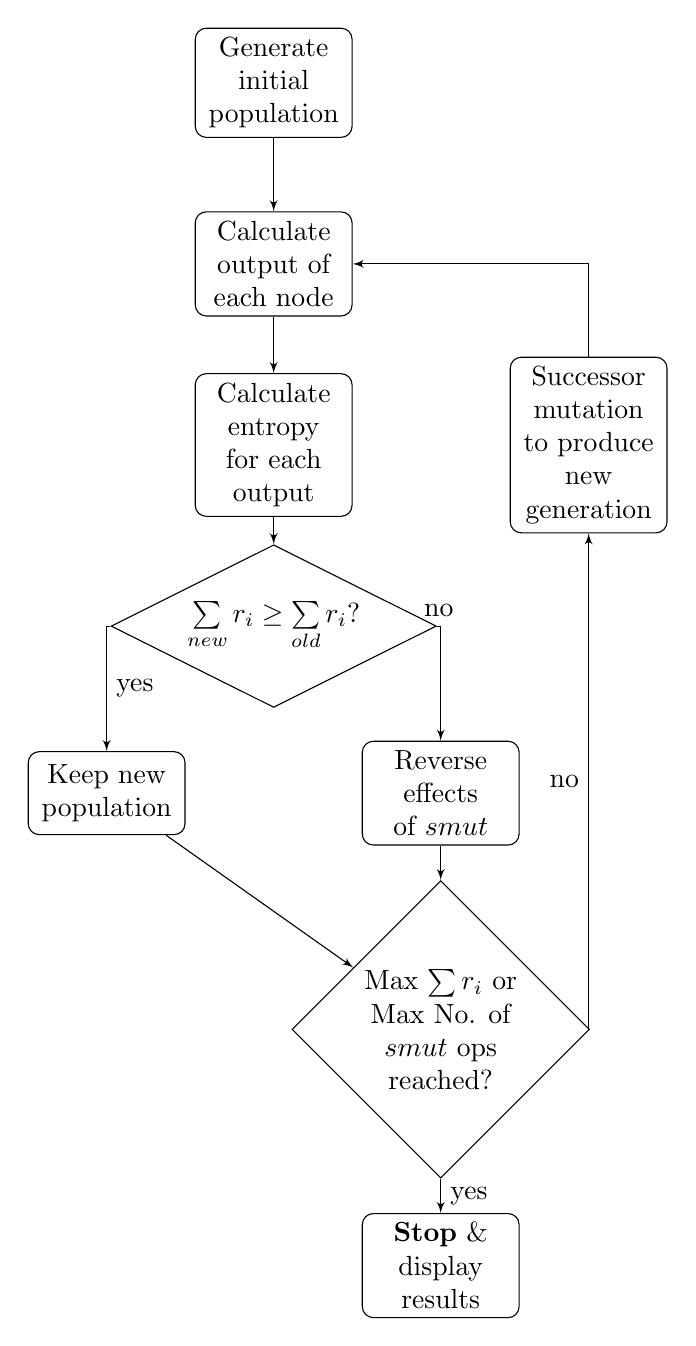
\begin{tikzpicture}[node distance = 2.3cm, auto]
    % Place nodes
    \node [block] (init) {Generate initial population};
    \node [block, below of=init] (identify) {Calculate output of each node};
    \node [block, below of=identify] (evaluate) {Calculate entropy for each output};
    \node [block, right of=evaluate, node distance=4cm] (update) {Successor mutation to produce new generation};
   
 \node [draw, diamond, aspect=2,  below of=evaluate] (decide1) {$\sum\limits_{new} r_i \geq \sum \limits_{old} r_i$?};
    \node [block, below left of=decide1, node distance=3cm] (greater) {Keep new population};
   \node [block, below right of=decide1, node distance=3cm] (less) {Reverse effects of $smut$};
    \node [decision, below of=less] (decide2) {Max $\sum r_i$ or Max No. of $smut$ ops reached?};
    
\node [block, below of=decide2, node distance=3cm] (stop) {\textbf{Stop} \& display results};
    % Draw edges
    \path [line] (init) -- (identify);
    \path [line] (identify) -- (evaluate);
    \path [line] (evaluate) -- (decide1);
    \path [line] (decide1) -| node  [near end]{yes} (greater);
    \path [line] (decide1) -| node [near start] {no} (less);
    \path [line] (less) -- (decide2);
    \path [line] (greater) -- (decide2);
    \path [line] (decide2) -| node [near end] {no} (update);
    \path [line] (update) |- (identify);
    \path [line] (decide2) -- node {yes}(stop);
\end{tikzpicture}
\end{wrapfigure}

A population is a set $M$ of $N$ members where;
\begin{center}
$M = \{m_0,\ m_1,\ ...,\ m_{N-1}\}$
\end{center}
Each member $m_i$ is a tuple;

\begin{center}
$m_i = \ <u_i,\ r_i,\ S_i,\ P_i,\ O_i>$
\end{center}
where;
\begin{center}
$u_i \in \{T \cup F\}$ - node in the terminal or function set\\
$r_i$ - fitness of the node\\
$S_i$ - set of successors of the node\\
$P_i$ - set of predecessors of the node\\
$O_i$ - output vector for this node\\
\end{center}
This tuple will be adapted into a $struct$ in C like the GP program described above.

For this implementation, I will be adapting the fitness value $r_i$ into a vector $R_i$ \footnote{So that the output of the SNGP will be the same as the GP, giving me the option to compare approaches on scalar entropies}. The first element in the vector will be the total fitness $E_{total}$ and the rest of the elements will be the scalar entropy values from $E_1$ to $E_7$.

SNGP is node focused, this means that members of the population are not trees, but are single nodes which together create a larger graph structure.

Figure 6 shows a flowchart for the anticipated SNGP implementation. Here we can see that the main functions are similar to those of GP.
In SNGP, the initial population is also randomly generated but instead, members of the population are chosen as individual nodes.

The Inputs to the SNGP implementation are shown in figure \ref{inputparamsngp} on page \pageref{inputparamsngp}. There are less inputs for the SNGP implementation compared to the conventional GP implementation. The length of a run is the equivalent to the maximum number of generations for GP, where instead the program terminates after a certain number of smut operations. The terminating fitness value is taken from the sum of all fitness values in all the nodes of the population. The population size is the number of nodes in the SNGP graph population. This size remains constant from initial generation throughout the rest of the run.

The SNGP population differs from the tree structure of a single member in the GP population. While the arity of functions and terminals remain the same as of that in the GP implementation, each function and terminal may have more than one predecessor. Therefore every node in the population can act as a root node for a RNG, and a population therefore contains as many RNGs as there are nodes. The reason for this coming about is due to the way that the population is initialised and evolved.

To begin with, all of the terminals in $T$ are added to the population exactly once. From here on in over all the generations, these terminals remain the same. What changes are their predecessors. Once the terminals are added, the functions are now selected randomly and are added to the population where their operands are existing members of the population. During initialisation of the population, the output and the fitness of each individual is also assessed. As Jackson describes in \cite[p.52]{jacksonsngp2}, this is what gives rise to SNGPs efficiency.

As the first terminals are added, they are evaluated for their outputs and their fitness is subsequently calculated. In this implementation of SNGP, this process is almost identical to that of the GP implementation described above. The terminal is evaluated for all values of $J$ from $i = 1$ to $2^{14}$, and each output is stored in the vector $O_i$ for that node. From this output vector a binary sequence of length $J$ is generated from the LSB of each element in $O_i$. The fitness of that node is the total entropy for subsequences of length 1 to 7 in the binary sequence, using the same equation as in the GP approach;
\begin{center}
 $E_{total} = \sum_{h = 1}^{7} \left[ - \sum_{j} P_{(hj)}\ \log_2\ P_{(hj)} \right]$
\end{center} 

This fitness/entropy value is stored in $r_i$ for that node. The efficiency of SNGP arises from using the following form of dynamic programming; when functions are now added to the population and their successors are assigned, the output and fitness for these nodes are calculated from the output vectors of their successors in the set $S_i$, as opposed to calculating them from scratch.

In SNGP, evolution is driven by hill-climbing. This is that the fitness is taken as the sum across the whole population; $\sum r_i$. After evolution this sum is calculated again, and if it is greater (higher entropy) than the last, then this evolved population replaces the previous population, otherwise the old population is kept and the process is repeated. This means that entropy/fitness can only climb higher. The total fitness $\sum r_i$ will be initially set to $-1$ so that the initial randomly generated population will always achieve a higher total fitness.

\begin{figure}[H]
\centering
\caption{Input parameters}
\label{inputparamsngp}
\begin{tabular}{l*{6}{l}r}
Data Type             & Input description\\
\hline
Integer & Length of a run (number of $smut$ operations)\\
Integer & Population size (number of nodes)\\
Double & Total (i.e. sum of) target fitness value\\
\end{tabular}
\end{figure}

Evolution of a SNGP is not done by using the crossover operation like in the GP above, but instead uses the $smut$ or successor mutation operation. A member of the population (a node) is randomly selected, and one of the members in it's successor set is changed to another member of the population (still at a greater depth in the tree). As we can see in figure \ref{smutexample}, a member in the successor set for the root node ``+", is mutated from ``\%" to  ``2";

\begin{figure}[H]
\caption{Successor Mutation}
\label{smutexample}
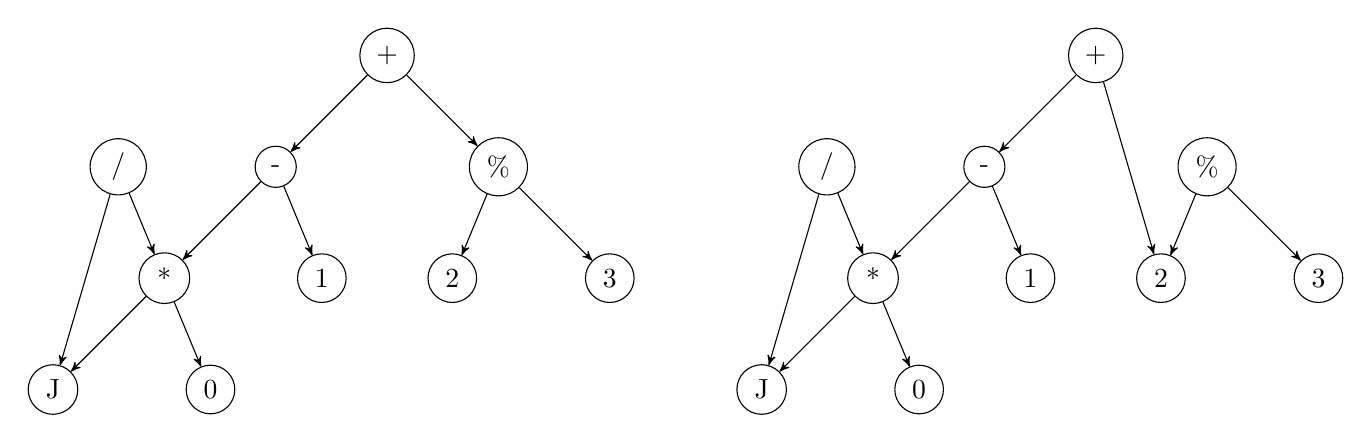
\begin{tikzpicture}[->,>=stealth',auto,node distance=2cm]

  \node[circle, draw] (+) {+};
  \node[circle, draw] (-) [below left of=+] {-};
  \node[circle, draw] (/) [left of=-] {/};
  \node[circle, draw] (*) [below left of=-] {*};
  \node[circle, draw] (mod) [below right of=+] {\%};
  \node[circle, draw] (J) [below left of=*] {J};
  \node[circle, draw] (0) [right of=J] {0};
  \node[circle, draw] (1) [right of=*] {1};
  \node[circle, draw] (3) [below right of=mod] {3};
  \node[circle, draw] (2) [left of=3] {2};

  \path[every node/.style={font=\sffamily\small}]
    (+) edge node [left] {} (-)
	 edge node [right] {} (mod)
        
    (-) edge node [right] {} (1)
	edge node [left] {} (*)
        
    (/) edge node [right] {} (*)
         edge node [left] {} (J)

    (*) edge node [left] {} (J) 
	edge node [right] {} (0)
        
    (mod) edge node [right] {} (3)
		edge node [left] {} (2);

\begin{scope}[xshift=9cm]
  \node[circle, draw] (+) {+};
  \node[circle, draw] (-) [below left of=+] {-};
  \node[circle, draw] (*) [below left of=-] {*};
  \node[circle, draw] (/) [left of=-] {/};
  \node[circle, draw] (mod) [below right of=+] {\%};
  \node[circle, draw] (J) [below left of=*] {J};
  \node[circle, draw] (0) [right of=J] {0};
  \node[circle, draw] (1) [right of=*] {1};
  \node[circle, draw] (3) [below right of=mod] {3};
  \node[circle, draw] (2) [left of=3] {2};

  \path[every node/.style={font=\sffamily\small}]
    (+) edge node [left] {} (-)
	 edge node [right] {} (2)
        
    (-) edge node [right] {} (1)
	edge node [left] {} (*)
        
    (/) edge node [right] {} (*)
         edge node [left] {} (J)

    (*) edge node [left] {} (J) 
	edge node [right] {} (0)
        
    (mod) edge node [right] {} (3)
		edge node [left] {} (2);
\end{scope}
\end{tikzpicture}
\end{figure}

In the example above, before mutation the population represents the prefix expressions (i.e. RNG trees);

\begin{center}
$\{J\}$, 
$\{0\}$, 
$\{1\}$, 
$\{2\}$, 
$\{3\}$, 
$\{* \ J \ 0\}$,
$\{/ \ J\ *\ J\ 0\}$, 
$\{-\ *\ J \ 0 \ 1\}$, 
$\{\%\ 2\ 3\}$,
$\{+\ -\ *\ J \ 0 \ 1 \ \%\ 2 \ 3\}$.
\end{center}
After the $smut$ operation it represents the following prefix expressions; \begin{center}$\{J\}$, $\{0\}$, $\{1\}$, $\{2\}$, $\{3\}$, $\{* \ J \ 0\}$, $\{/ \ J\ *\ J\ 0\}$, $\{-\ *\ J \ 0 \ 1\}$, $\{\%\ 2\ 3\}$, $\{+\ -\ *\ J \ 0 \ 1 \ 2\}$\end{center}

During $smut$, not all of the program nodes are effected, and therefore not all of them need to be reevaluated for their outputs and fitnesses. As Jackson describes in \cite[p.53]{jacksonsngp} SNGP retains it's efficient nature by creating an update list, where only nodes effected by smut are added. Nodes in the list are reevaluated starting at the lowest node in the list working up to the highest node so that no node is revisited.

The outputs for the SNGP implementation are almost identical to those of the GP. Instead of Generation Number, the output here will be the $smut$ operation count. The rest of the outputs will be the same as shown in figure \ref{outputparamsngp} below;

\begin{figure}[H]
\centering
\caption{Output data}
\label{outputparamsngp}
\begin{tabular}{l*{6}{l}r}
Data Type             & Output description\\
\hline
Integer & $smut$ operation count\\
Double & Generation run time in seconds \& hundredths of a second \\
Double & Entropy for subsequence size 1 of fittest candidate\\
\ \ \ \ $\vdots$ & \ \ \ \ \ \ \ \ \ \ \ \ \ \ \ \ \ \ \ \ \ \ \ \ $\vdots$\\
Double & Entropy for subsequence size 7 of fittest candidate\\
Double & Total entropy/fitness of fittest candidate\\
Boolean & Entropy of fittest candidate is $\geq$ target fitness?\\
String & Prefix expression for fittest candidate
\end{tabular}
\end{figure}

The fittest candidate (i.e. best RNG tree) in a SNGP population is the tree where the root node has the maximum $R_i$ across the whole population. This prefix expression is what is used to output to the file above in figure \ref{outputparamsngp}

Above is a literal description of the design for the SNGP implementation. A pseudocode for the key methods in the implementation can be created from the definitions above. Algorithms  4, 5 and 7 in section 2.1 are synonymous with the GP and the SNGP implementations. What differs where and when these algorithms are called, and how their outputs are stored. Algorithms 8, 9 and 10 below cover the altered and extra main methods in the SNGP implementation.

\begin{algorithm}[H]
  \caption{Generate-Initial-SNGP-Population($M_{s}$, $T$, $F$, $J$)}
  \textbf{Input:} Population size $M_{s}$, set $T$ of terminals and set $F$ of functions, Integer $J$\\
  \textbf{Output:} Population $M$ of randomly generated programs of size $M_s$\\
  \begin{algorithmic}[1]
    \State $i \gets 1$
    \For {$i$ to $M_{s}$} 
	\If {$T \neq \emptyset$}
		\State $node = $random $x \in T$
		\State $M \cup node$ 
		\State $T = T - node$
	\Else
		\State $node = $random $ x \in F$
		\State $j \gets 0$
		\For {$j$ to $node.arity$} 
			 \State $p \gets $random $y \in M$
			 \State $P_p \cup node$
			 \State $S_{node} \cup p$
		\EndFor\\

		\State $T \gets $ Get-Tree($node$, $\varepsilon$)
		 \For {$i \gets 0$ to $J$}
			\State $O_{node}[i] \gets$ Evaluate-Tree($T_0$, $i$)
			\State $BinSeq[i] \gets O_{node}[i] \mod 2$
 		\EndFor
		\State $R_{node} \gets $ Fitness-Function($BinSeq$)
		
		\State $M \cup node$
	\EndIf

    \EndFor	
\State \textbf{return} $M$
  \end{algorithmic}
\end{algorithm}

\begin{algorithm}[H]
  \caption{Get-Tree($root$, $T$)}
  \textbf{Input:} Root node of tree $root$, existing tree prefix expression $T$\\ 
  \textbf{Output:} Modified tree prefix expression $T$\\

  \begin{algorithmic}[1]
   \State $T = T + root$
  \If {$S_{root} \neq \emptyset$}
	\State $left \gets $ left node of $S_{root}$ for $root\in M$
	\State $T \gets $ Get-Tree($left$, $T$)
	\State $right \gets $ right node of $S_{root}$ in $root\in M$
	\State $T \gets $ Get-Tree($right$, $T$)
   \EndIf
\State \textbf{return} $T$
  \end{algorithmic}
\end{algorithm}

\begin{algorithm}[H]
  \caption{Successor-Mutation($m_i$)}
  \textbf{Input:} Randomly selected member of the population, where $m_i \notin T$\\ 
  \textbf{Output:} $m_i$ with modified successor set\\

  \begin{algorithmic}[1]
   \Repeat
	\State $newSuc \gets$ random $x \in M$
   \Until {$newSuc.depth > m_i.depth$}
   \State $S_i - random \ x \in S_i$
   \State $S_i \cup newSuc$
   \State \textbf{return} $m_i$
  \end{algorithmic}
\end{algorithm}

\newpage
\subsection{System Evaluation Design}
Due to the thoroughness of data collection for both GP and SNGP in the designs above, there exists a variety of methods at my disposal in order to evaluate the project. Referring to the third point of the project objectives in section 1 of this document, we can see that the success of the software will be determined on two main evaluation premises.
Primarily we shall design an evaluation, comparing the GP implementation against the SNGP implementation, which will use the data gathered across many runs of both.
Secondly I shall design a comparison of the fittest GP and SNGP generated RNG trees against a widely used PRNG and also against a TRNG, again determining their randomness using a fitness function, calculating the entropy of a random binary sequence.

\subsubsection{GP vs SNGP}
In order to compare the GP and SNGP approaches, we must run the same input cases on both to obtain a set of outputs. To create these input cases we must only select the inputs which are synonymous between the two approaches and then leave the rest as a constant throughout all of the cases. Figure \ref{inputforboth} below shows the matching input parameters between both implementations;

\begin{figure}[H]
\centering
\caption{Matching parameters}
\label{inputforboth}
\begin{tabular}{l*{6}{l}r}
Data Type             & Input description\\
\hline
Integer & Maximum number of generations / Length of a run (number of $smut$ operations)\\
Integer & Population size; number of trees (GP) or number of nodes (SNGP)\\
Double & Target fitness value (GP), Target fitness value for sum of all node targets (SNGP) \\
\end{tabular}
\end{figure}

The remaining input parameters are only in the GP implementation. Figure \ref{loparam} below shows the leftover parameters and their values\footnote{These values are the ones which are defined by Koza in \cite[p.41]{kozarng}} across all test cases for the GP implementation;
\begin{figure}[H]
\centering
\caption{Remaining constant parameters for GP}
\label{loparam}
\begin{tabular}{l*{6}{l}r}
Data Type             & Input description & Values\\
\hline
Integer & Maximum initial program depth & 4\\
Integer & Maximum crossover program depth & 15\\
Double & Fitness proportionate reproduction probability & 0.1\\
Double & Crossover operation probability & 0.9\\
Double & Internal node crossover probability & 0.9\\
Double & External node crossover probability & 0.1\\
\end{tabular}
\end{figure}

For figure \ref{inputforboth} we must define a set of test cases concerning the values of these parameters. For each input I want to test it for a regular case and for an intensive case. For Maximum Generations/$smut$ operations I want to test for a regular limit of 51 to a larger limit of 101. For Population size, I want to test it for a regular limit of 500 to a larger size of 1000. For the Target fitness, I want to test it for a regular entropy of 27.990 as described by Koza in \cite[p.41]{kozarng}, and a perfect fitness score of 28 (for SNGP this input value will be multiplied by that test cases population size). All combinations of these inputs give us $p$ (possible values of each input) and $k$ (the number of inputs), $p^k = 2^3 = 8$ test cases shown in the matrix below;
\begin{equation*}
\text{Test Matrix} = \bordermatrix{~ &  1&  2& 3& 4& 5 & 6 & 7 & 8\cr
                  $Max Gen/$smut& 51 & 51 & 101 & 101& 101 & 101 & 51 & 51   \cr
                  $Pop size$& 500 & 1000 & 500 & 1000 & 500 & 1000 & 500 & 1000  \cr
	       $Targ Fit$ & 27.990 & 28.0 & 27.990 & 28.0 & 28.0 & 27.990 & 28.0 & 27.990 \cr}
\end{equation*}

Now that we have created test cases, both GP and SNGP will be run on these test cases which will generate time stamped files containing there respective outputs. Each test case can be run a number of times in order to produce outputs that we can average. 

The fitness data and various properties of the program runs (i.e. average run time) can be used to pit the SNGP and GP against each other to determine which method performs best. For my evaluation I shall be comparing SNGP and GP using the following criteria;

\begin{description}
  \item[1)]
  \ \ Average entropy fitness of fittest member over 100 runs
  \item[2)]
 \ \ Average solution rate over 100 runs
  \item[3)]
 \ \  Average minimum and maximum solution size over 100 runs
  \item[3)]
  \ \ Average run time over 100 runs
  \item[4)]
  \ \ Generation run time over one run
  \item[5)]
  \ \  Average solution size over one run
  \item[6)]
  \ \  Entropy climb over one run
  \item[7)]
  \ \  Scalar entropies over one run
\end{description}

There are also a variety of ways in which these comparisons can be represented in both visual and descriptive ways.

For my evaluation, I shall mainly be using charts to compare the statistics for both GP and SNGP outputs, and discussing their implications in terms of which method is best suited for their application. An example graph can be seen below in figure \ref{examplegraph}, comparing both SNGP and GP methods on a single run for the first test case in the matrix above;

\begin{figure}[H]
\caption{Example evaluation graph}
\label{examplegraph}
\begin{tikzpicture}
\begin{axis}[width=\textwidth]
\addplot table [x=a, y=b, col sep=comma] {data.dat};
\addplot table [x=c, y=d, col sep=comma] {data.dat};
\addplot [dash pattern=on 1pt off 3pt] table [x = e, y = f,  col sep=comma] {data.dat};
\addplot [dash pattern=on 1pt off 3pt] table [x = g, y = h,  col sep=comma] {data.dat};
\end{axis}
%\draw node [above] {};
\draw node [label={[label distance=11.5cm]85:Max Entropy = 27.990}] {};
\draw node [label={[label distance=13.8cm, rotate=-90]93:Max Gen \# or $smut$ operations = 51}] {};
\draw node [label={[label distance=7.5cm]48:SNGP}] {};
\draw node [label={[label distance=7.5cm]27:GP}] {};
\end{tikzpicture}
\end{figure}

After comparison of both approaches, the expected result is that SNGP will outperform GP in most if not all evaluation criteria. The reason for this is that comparisons of the two methods conducted by Jackson in \cite[p.55]{jacksonsngp} display SNGP superiority over GP. As the fitness function and tree evaluation are computationally intensive (and a possible bottleneck for both approaches), SNGPs use of dynamic programming for both calculations should see it's run time substantially reduced in comparison to the GP implementation.


\subsubsection{Other Random Number Generators}
After methods for generating RNGs using GP have been evaluated, the actual RNGs produced should be compared to a widely used Pseudo Random Number Generator and a True Random Number Generator.

In order to evaluate these other RNGs, the same fitness function will be used so as to determine their randomness in terms of entropy. Therefore evaluation criteria will strictly be concerned with entropy as all the other criteria as described above are concerned with the GP functions.

\subsubsection{C Rand function}
The rand() function used in the C programming relies on the use of a PRNG. In order to calculate it's entropy, I shall write a small C program which call this function $i = 0$ to $J$ times, each time finding the LSB of it's output and again populating a binary output vector. This vector can then be assessed for it's entropy using the same fitness function as in Algorithm 5 in section 2.1.1. This process will be repeated a number of times to obtain an average total entropy value and scalar entopies, which can be can then be compared to the fittest RNG produced by the GP/SNGP method.

\subsubsection{True Random Number Generator comparison}
As described in the specification document, a TRNG is a random number generator which employs a piece of hardware to generate a random number. As these pieces of hardware can be expensive and hard to come by I shall be making use of the free TRNG at http://www.random.org/. Random binary sequences at random.org are produced using a piece of hardware which measures atmospheric noise. This service allows users to make use of a free 1,000,000 bit quota per IP address (with a 200,000 bit top up each day to refill the 1,000,000 quota). These sequences are available over the Hyper Text Transfer Protocol (HTTP), therefore I shall be writing another simple C program to request a binary sequence of length $J$ over HTTP. The program will then extract the data from the packet and determine the sequences fitness using the same fitness function in Algorithm 5 to determine it's entropy and scalar entropies. I shall repeat this process a number of times (remembering that $\lfloor\frac{1,000,000}{J} \rfloor$= 61 tests) to obtain an average entropy produced by the TRNG.
Using this information I can then compare it with the entropy of the fittest RNG produced by the GP/SNGP method. \\

\noindent Using all of these evaluation methods will give a clear conclusion to;
\begin{description}
  \item[a)] Which method of Generating Random Number Generators using Genetic Programming is most successful and;
\item[b)] Whether the best RNGs produced by these approaches are a viable option compared to other (non genetically evolved) RNGs
\end{description}

\section{Plan Progress}
The progress of the project is going well, no rearrangements or readjustments need to be made to the Gantt chart, just the movement of the current date in order to show what aspects of the project have been completed. These are namely, the Specification, Research and the Design, and so reaching the milestone ``Implementation documentation complete".

The next stage to the project after the presentation is implementation, specifically the implementation of the GP approach. I shall be using the algorithms described in section 2.1 to write the program in C.\\

\noindent Please See figure~\ref{fig:ganttchart} on page~\pageref{fig:ganttchart} for the up to date Gantt Chart

\begin{sidewaysfigure}

\centering
\begin{ganttchart}[y unit title=0.4cm,
y unit chart=0.5cm,
vgrid,hgrid, 
title label anchor/.style={below=-1.6ex},
title height=1,
bar/.style={fill=gray!50},
bar/.append style={fill=gray!100},
bar incomplete/.append style={fill=gray!50},
incomplete/.style={fill=white},
progress = today,
today = 10, 
bar height=0.7,
group right shift=0,
group top shift=.6,
group height=.3,
group peaks height =.2,
milestone/.append style={fill=gray!50}
]
{1}{34}
%labels
\gantttitle{Final Year Project}{34} \\
\gantttitle{Sep}{2} 
\gantttitle{Oct}{4} 
\gantttitle{Nov}{4} 
\gantttitle{Dec}{4} 
\gantttitle{Jan}{4} 
\gantttitle{Feb}{4} 
\gantttitle{Mar}{4} 
\gantttitle{Apr}{4} 
\gantttitle{May}{4} \\
%tasks
\ganttbar{Research}{1}{6} \\
\ganttgroup{Specification}{2}{4} \\
\ganttbar{Write Specification}{2}{4} \\
\ganttgroup{Design}{5}{10} \\
\ganttbar{Plan Design}{5}{5}\\
\ganttbar{Write Design Document}{6}{9}\\
\ganttbar{Plan Presentation}{9}{9}\\
\ganttbar{Give Design Presentation}{10}{10} \\
\ganttmilestone{Implementation Documentation Complete}{10}\\
\ganttgroup{Implementation}{11}{26} \\
\ganttbar{Implement Koza's PRNG GP}{11}{18}\\
\ganttbar{Implement SNGP Approach}{19}{23} \\
\ganttbar{Compare GP vs SNGP}{24}{26}\\
\ganttmilestone{Implementation Complete}{26} \\
\ganttgroup{Demonstration}{27}{28} \\
\ganttbar{Write/Plan Demonstration}{27}{27} \\
\ganttbar{Give Demonstration}{28}{28} \\
\ganttgroup{Dissertation}{29}{34} \\
\ganttbar{Plan Dissertation}{29}{29}\\
\ganttbar{Write Dissertation}{30}{34} \\
\ganttmilestone{Project Completed}{34} \\

%relations
\ganttlink[link type=dr]{elem2}{elem4} 
\ganttlink[link type=dr]{elem4}{elem5}
\ganttlink[link type=dr]{elem4}{elem6}
\ganttlink[link type=dr]{elem5}{elem8}
\ganttlink[link type=dr]{elem6}{elem7}
\ganttlink[link type=dr]{elem7}{elem8} 
\ganttlink[link type=dr]{elem8}{elem10} 
\ganttlink[link type=dr]{elem10}{elem11}
\ganttlink[link type=dr]{elem10}{elem12}
\ganttlink[link type=dr]{elem11}{elem12}
\ganttlink[link type=dr]{elem12}{elem13} 
\ganttlink[link type=dr]{elem13}{elem15}
\ganttlink[link type=dr]{elem15}{elem16}
\ganttlink[link type=dr]{elem16}{elem18}
\ganttlink[link type=dr]{elem18}{elem19}
\ganttlink[link type=dr]{elem19}{elem20}

\end{ganttchart}
\caption{Gantt Chart - Work plan}
\label{fig:ganttchart}
\end{sidewaysfigure}

\newpage 

\begin{thebibliography}{10}

\bibitem{kozarng}
  John R. Koza, 
  \emph{Evolving a Computer Program to Generate Random Numbers Using the Genetic Programming Paradigm}. 
  Stanford University, 
  1991.

\bibitem{jacksonsngp}
  David Jackson,
  \emph{Single Node Genetic Programming on Problems with Side Effects}.
  University of Liverpool,
  2012.

\bibitem{mitchell}
  Melanie Mitchell,
  \emph{An Introduction to Genetic Algorithms}.
  MIT Press,
  1999.

\bibitem{lapantebio}
  Phillip A. Laplante,
  \emph{Biocomputing}.
  Nova Science Publishers Inc,
  2003.

\bibitem{introgp}
  R. Poli, W. B. Langdon, N. F. McPhee, J. R. Koza, 
  \emph{A Field Guide to Genetic Programming}. 
  University of Essex, 
  2008.

\bibitem{kozagpbook}
  John R. Koza, 
  \emph{Genetic Programming. On the Programming of Computers by Means of Natural Selection}. 
  MIT Press, 
  1992.

\bibitem{kozamux}
  John R. Koza,
  \emph{A Hierarchical Approach to Learning the Boolean Multiplexer Function}
  Stanford University,
  1990.

\bibitem{cprog}
  Brian W. Kernighan, Dennis M. Ritchie, 
  \emph{C Programming Language}.
  2nd Edition, 
  Prentice Hall Professional Technical Reference, 
  1988.

\bibitem{jacksonsngp2}
  David Jackson,
  \emph{A New, Node-Focused Model for Genetic Programming}.
  Proceedings of the 15th European Conference on Genetic Programming, EuroGP 2012, 
  Springer Verlag
  2012.

\bibitem{prnggp}
  C. Lamenca-Martinez, J.C. Hernandez-Castro,
  J.M. Estevez-Tapiador, and A. Ribagorda
  \emph{Lamar: A New Pseudorandom Number Generator Evolved by means of Genetic Programming}.
  University of Madrid,
  2006.

\bibitem{entropy}
  Robert M. Gray
  \emph{Entropy and Information Theory}.
  First Edition (Corrected),
  Stanford Unviersity
  2000.

\end{thebibliography}

\end{document}